\chapter{Literature Review} \label{chap:bib} %% chapter 3

\section {Wi-Fi}
\hspace {5mm} 

Wi-Fi is a technology for implementing wireless area networks. In these networks, devices like computers, smartphones, are connected via wireless access points and a WLAN. The first version of the protocol was released in 1997, and since then, it was adopted internationally.   

\par The specifications are set in the IEEE 802.11 standard. This is a set of specifications that complying devices need to meet in order to provide connectivity. Encompassing several standards, each one extending the functionality, and improving the physical layer of the transmission channel. The first widely accepted standard, 802.11b uses the 2.4 GHz band, and supporting up to 14 channels, suffered from the effect of interfering products using this band, such as Bluetooth devices, and microwaves. Published in 2013, 802.11ac is the most current protocol, and this evolution brought the 5 GHz band, and faster transmission speeds. Deployment of these different standards vary in technical requirements and budget constraints.

\par The common access method from the devices are the wireless access points (WAP). They enable the communication in the network, and is at its best when supporting from 15 to 25 clients, and, while designing the system, the usage of the system should consider the amount of users and devices that access the network. Taking in account these considerations, we can start defining what requirements need to be considered when designing large scale networks, for example in enterprises or school networks, where the need for permanent connection is paramount. 

\par The increasing demand for larger WLAN's everywhere also imposes other, just as important requirements, like security, mobility support, among others. The scaling of the resources brings a necessity that doesn't exist in traditional configurations, because the management is traditionally centralized, and the systems are usually proprietary, bringing several difficulties to the configuration of the systems.

%% CITE THIS SHIT
\begin{figure}
    \centering
    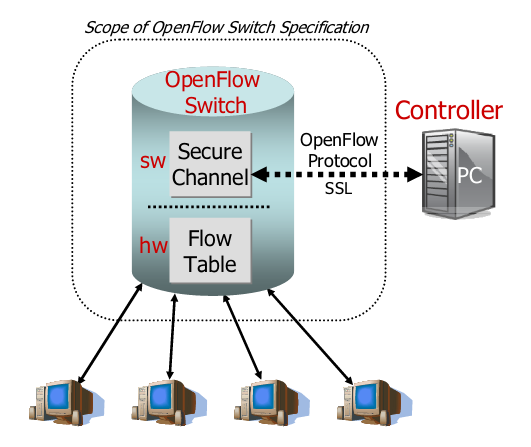
\includegraphics[scale=.4]{openflow}
    \caption{
        The ideal openflow switch \cite{mckeown_openflow:_2008}
    }
    \label{fig:my_label}
\end{figure}

\par Taking into account these considerations, a solution that could solve these issues needs to be developed. Therefore, by using the recent concepts of \textbf{ Software Defined Networks} (SDN), and \textbf{Network Function Virtualization} (NFV), we can start exploiting the features these paradigms offer us. SDN is a concept of abstraction of the physical level of networking, that allows for administrators to manage networks programmatically, by creating a virtual controller that enables a centralized configuration and faster evolution of the network, either by allowing a quicker deploy and configuration time, or by developing a faster way to detect errors in the operation of the service. 

\par One proposal to implement this system, on a college campus, is \textbf{openflow}, which design we inserted in the previous figure. The necessity of implementing a way to experiment with networks on college campus, for testing of new ideas was big, so they solved this issue by implementing a system that is transparent to vendor software, and can isolate the experimental traffic from production traffic. 

\par The other innovation that, in a way, was possible due to the concept of SDN is NFV \cite{schulz-zander_opensdwn:_2015}. By virtualizing the function of hardware switches, routers, we can guarantee the requirements of the networks are met. One of the larger requirements for this is the logical infrastructure supporting these networks, and developments in cloud computing allowed for bigger and better solutions. 

\par In the next sections we will define requirements to some of the previously mentioned topics, and specific technologies that allow to meet these resources. 

\subsection {Wi-Fi session information}
\hspace {5mm}

AAA stands for Authentication, Authorization and Accounting, and is one of the primary systems that should be accounted for in the design of large scale WLAN, and they are one of the factors allowing for the support of mobility across networks, and dynamically supporting security. In this system, a client connects to an authenticator, and, according to it's decision, the user information is stored in an accounting storage. This accounting manager is what enables the system to provide mobility across systems, since this plane is separated from the AP which the client is associated with. The accounting service is commonly powered by cloud computing layers, and its aspects are described further in this chapter.

\par Other type session information vital to these infrastructures is explored in a research done by Allahdadi et al. \cite{allahdadi_predicting_2013}, and they focus their work on analyzing network usage in time scales lower than 5 minutes. By modeling aspects of these connections, they check the amount of users and the amount of time of their sessions, and this was able to give information on the poor network performance associated with these connections. This information is vital to our work since it has insight on what information should be prioritized. 

\par Also to be taken into consideration is information about each user MAC and the respective AP MAC address, duration, bytes transmitted and received, and the number of packets in the session.

\subsection {Managed Wi-Fi}
\hspace {5mm}

The big paradigm that allows for the implementation of the above systems in Managed Wi-Fi Networks. Solutions such as Cisco's Meraki, Ubiquiti UniFi are systems that leverage the power of cloud computing, in order to provide in their systems a solution that allow for providing to the system administrators a highly reliable system, often removing problems that enterprises face, that is reduced physical space for the storage of networking hardware, or even the lack of available on-site support teams, in case of necessary troubleshooting. 

\par Requirements for these services are:

\begin{itemize}
    \item The optimization for wireless coverage, both in aspects of expected usage and facility design;
    \item Multiple authentication options, needed when the system needs to support different types of traffic, such as guests or customers
    \item And support the requirements for security, such as WPA key rotation 
\end{itemize}

%% OPENSDWN

OpenSDWN \cite{schulz-zander_opensdwn:_2015} is an architecture in deploying a Wi-Fi architecture that meets these requirements. By extending Odin, this system allows for the deployment of systems that feature the above characteristics.


\section {Cloud Computing}
\hspace {5mm}

Supporting the integration of SDN Wi-Fi are cloud computing infrastructures, and these will be essential to the performance needed to achieve proper functioning networks. In the scope of the future thesis is to research the possible advantages of the multiple solutions of cloud computing offered like Amazon Web Services or Azure.

\par For this document, however, we focused on \textbf{OpenStack} \cite{callegati_performance_2014}, and how they impact the performance of Virtual Networks. This research is based on the work done here, and they setup the networking component of OpenStack, Neutron, and this allowed for the solution of two problems, the integration of the virtual controllers, and the logic imposed isolation necessary to the segregation of traffic. 

\section {Databases}
\hspace {5mm}

From the analysis of the requirements of the previous sections, the database design is a requirement to support all of these systems, and the choice of this system is core to the correct performance of the system. We then need to find the amount of data that is generated and collected from the underlying system, and also choose what database system has the best possible performance that suits our needs.

\par The most common databases are \textbf{Structure Query Language (SQL)} databases, and PostgreSQL or MySQL are the most common used languages in the relational database world, and the widespread use of these databases provides a large amount of content of research. The recent surge of popularity, backed in part by Amazon or Google, of \textbf{NoSQL} languages, used mostly in bigdata applications, must also be considered in the scope of our research. One of the steps of our work is to analyze the different performance of several databases in the different operations that can be done, writing, reading, searching, among others. Research on this topic was done by Yishan Li and Sathiamoorthy Manoharan \cite{li_performance_2013}, which tested the performance of different databases, and this analysis showed that different performances were obtained, so, the choice of database must be done by analyzing the data, and finding a balance to our system.

\par The first step, during the development of our work, should then be the analysis of the session information, introduced previously in this chapter, and also the creation of a structured model that best fits our findings. 

